\question{Ein Pfeil wird auf eine Zielscheibe geschossen und bleibt stecken. Warum fliegt das Endstück Rückwärts weg?}

Fig TODO Dominik

\begin{tasks}(1)
    \task[$\bullet$] Skizzieren Sie den Kraft- und Geschwindigkeitsverlauf im Pfeil (Dehnstab)
    \task[$\bullet$] Vergleichen sie Ihr Ergebnis mit einem Einmassenschwinger, der gegen die Wand fliegt.
\end{tasks}

\begin{solution}
\flushleft HIER BITTE NOCH LÖSUNG NACHTRAGEN (Dominik Kern)
\end{solution}

\question{Ein halbunendlicher Stab wird am Rand harmonisch angeregt.

\vspace{1cm}

\begin{figure}[h]
    \centering
    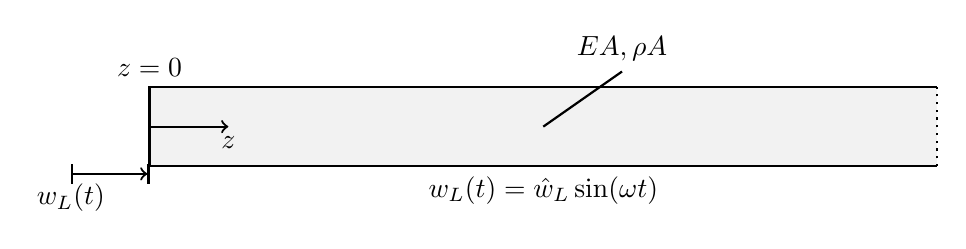
\begin{tikzpicture}
        \draw[thick, fill=gray!10] (10,0) -- node [midway, below] {$w_L (t) = \hat{w}_L \sin(\omega t)$} (0,0) -- (0,1) node[above] {$z=0$} -- (10,1) ;
        \draw[thick, dotted] (10,0) -- (10,1);
        %\draw[thick, ->] (10,0.5) -- (11,0.5);
        \draw[thick, ->] (0,0.5) -- (1,0.5) node[left, below] {$z$} ;
        \draw[thick, |->|] (-1,-0.1) node[below] {$w_L (t)$} -- (0,-0.10);
        \draw[thick] (5,0.5) -- (6,1.2) node[above] {$EA,\rho A$};
    \end{tikzpicture}
\end{figure}


Am Anfang $(t=0)$ ist er undeformiert und in Ruhe. Lösen Sie diese Aufgabe, indem Sie auf dem gedanklich über den Rand verlängerten Stab eine nach rechts laufende Welle annehmen, welche genau die vorgegebene Randbewegung erzeugt. Interpretieren Sie die Parameter dieses Verlaufs physikalisch, Stichwort ``Wellenlänge".
}

\begin{solution}
    
    \begin{align*}
        \intertext{Aus dem D'alembertschen Wellenansatz mit $t = 0$}
        &w_0(z) = \Psi(z) + \Phi(z)
        &\dot{w_0}(z) = c\Psi^{'}(z)-c\Psi^{'}(z)
        \intertext{folgt:}
        &\Psi(z) = C_1 \cos(\kappa z) + C_2 \sin(\kappa z)
        &\Phi(z) = R_1 \cos(\kappa z) + R_2 \sin(\kappa z)
    \end{align*}
\end{solution}

\question{Berechnen Sie das Reflektionsverhalten diskreter Elemente am Rand: Feder, Dämpfer und Masse.

\begin{tikzpicture}[scale=0.6]
\fill[black!25!white] (4,-1.5) rectangle +(1.5, 3); 
\fill[black!10!white] (5.5,-0.5) rectangle +(5.5, 1);  
\draw (0, 0) pic [scale=0.6] {DKbase};
\draw (0, 1) pic [scale=0.6, thick] {DKspring=4};
\draw (0,-1) pic [scale=0.6, thick] {DKdashpot=4};  
\draw[thick] (4,-1.5) rectangle +(1.5, 3); 
\draw[thick] (5.5, -0.5) -- (11, -0.5);
\draw[thick] (5.5,  0.5) -- (11,  0.5);
\draw (2.0, 0.1) node {$k$};
\draw (2.0,-1.9) node {$c$};
\draw (4.75, 0) node {$m$};
\draw (8, 0) node {$E$,$A$,$\rho$};
\end{tikzpicture}


Nehmen Sie dazu eine einfallende nach links laufende Welle $w_{ein}(z,t) = C_1 \cos(kz+\omega t)$ an und 
berechnen Sie die reflektierende Welle $w_{ref}(z,t)=R_1\cos(kz-\omega t) + R_2 \sin(kz-\omega t)$. \\
\qquad

\fbox{Hinweis ($z=0$):}
\begin{tasks} (3)
    \task[] $kw = EAw'$
    \task[] $c\dot w = (EA)w'$
    \task[] $m\ddot w = (EA)w'$
    \task[] Feder-RB
    \task[] Dämpfer-RB
    \task[] Masse-RB
\end{tasks}

\fbox{
    \begin{minipage}[t]{\textwidth}
        Hinweis: Der Punkt steht für die Ableitung nach der Zeit $t$, \\der Apostroph für die Ableitung nach der räumlichen Koordinate $z$.
    \end{minipage}}
}    

\begin{solution}
        Ableitungen der Funktion $w$:
        \begin{align*}
            \dot{w} &= -C_1 \omega \sin(\kappa z + \omega t) + C_2 \omega \cos(\kappa z + \omega t) \\
                     &+ R_1 \omega \sin(\kappa z - \omega t) - R_2 \omega \cos(\kappa z - \omega t) \\
            \ddot{w} &= - C_1 \omega^2 \cos(\kappa z + \omega t) - C_2 \omega^2 \sin(\kappa z + \omega t) \\
                     &-R_1 \omega^2 \cos(\kappa z - \omega t) - R_2 \omega^2 \sin(\kappa z - \omega t) \\
            w^{'} &= -C_1 \kappa \sin(\kappa z + \omega t) + C_2 \kappa \cos(\kappa z + \omega t) \\
                   &-R_1 \kappa \sin(\kappa z - \omega t) + R_2 \kappa \cos(\kappa z - \omega t)
        \end{align*}

        Schrittweise Berechnung der Reflektion: \\
        1. Anfangsbedingung: $z=0$ \\
        2. Ausklammern der Sinus- und Cosinus-Ausdrücke (am besten in Matrixform)\\
        3. Aus den erhaltenen Koeffizienten der Sinus- und Cosinusfunktionen kann nun nach $R_1$ und $R_2$ umgestellt werden.
            Dabei ergibt sich $R_1$ aus den Koeffizienten des Kosinus und $R_2$ aus den Sinuskoeffizienten.\\

        Feder:
        \begin{align*}
            0 &= kw - EA  w^{'}\\
            R_1 &= \frac{C_1 {(EA)}^2 \kappa^2 - C_1 k^2 + 2C_2 (EA) k \kappa}{{(EA)}^2 \kappa^2 + k^2}\\
            R_2 &= \frac{2C_1 (EA) k \kappa - C_2 {(EA)}^2 \kappa^2 + C_2 k^2}{{(EA)}^2 \kappa^2 + k^2}
        \end{align*}
        Dämpfer:
        \begin{align*}
            0 &= c \dot{w} - EA  w^{'}\\
            R_1 &= \frac{C_1 (EA) \kappa - C_1 c w}{(EA) \kappa + cw}\\
            R_2 &= \frac{-C_2 (EA) \kappa + C_2 cw}{(EA) \kappa + cw}
        \end{align*}
        Masse:
        \begin{align*}
            0 &= m \ddot{w} - (EA) w^{'}\\
            R_1 &= \frac{C_1 {(EA)}^2 \kappa^2 - C_1 m^2 \omega^4 - 2C_2 (EA) \kappa m \omega^2}{{(EA)}^2 \kappa + m^2 \omega^4}\\
            R_2 &= \frac{-2C_1 (EA) \kappa m \omega^2 - C_2 {(EA)}^2 \kappa^2 + C_2 m^2 \omega^4}{{(EA)}^2 \kappa + m^2 \omega^4}
    \end{align*}
\end{solution}

\question{Resonant Column}
TODO Dominik Kern (siehe V09aufgaben.pdf) stehende Welle

\vspace{1cm}

\begin{tikzpicture}
\draw[thick, fill=black!10!white] (-0.2, 0) rectangle (0.2, 3.0);
\draw[thick, fill=black!20!white] (-0.5, 3) rectangle (0.5, 3.5);
\draw(1, 3.2) node[right] {$J$};
\draw(1, 1.5) node[right] {$G,I,\rho$};
\draw (0, 0) pic [rotate=90, scale=0.5] {DKbase};
\draw[<->, thin] (-0.4, 0) -- node[left] {$l$} (-0.4, 3);
\draw[thin] (0.1, 1.0) -- (1.0, 1.5);
\draw[thin] (0.4, 3.3) -- (1.1, 3.2);
\end{tikzpicture}

